%!TEX TS-program = xelatex
%!TEX root = ../../maxwell2018thesis.tex

\begin{preamble}[Presentational Conventions]
\phantomsection
\addcontentsline{toc}{part}{Presentational Conventions}

A number of different presentational conventions have been employed in this thesis for a consistent (and different) look, and to maximise understandability. This section outlines the conventions that have been used.

\glsunset{acr:url}


\noindent\blueboxbold{Spelling}
\begin{itemize}
    \item{Spelling is according to the \emph{Oxford English Dictionary} (British English). The version that was referred to is searchable online at \url{https://en.oxforddictionaries.com/}. We prefer a \emph{s} to a \emph{z}!}
\end{itemize}

\noindent\blueboxbold{Fonts and Emphasis}
\begin{itemize}
    \item{\emph{Italicised text} is used to define a term and/or concept, but not thereafter. This applies to acronyms, where the full expansion is presented initially; associated abbreviations are used thereafter. Full expansions of an acronym may be reused if required (i.e. in later chapters).}
    
    \item{The main body of this thesis is typeset in 12-point Palatino (body) with 1\sfrac{1}{2} line spacing. Headers, figures and tables (along with their associated captions) use \headerfont\selectfont Foundry Sterling\normalfont\selectfont. The names of tools used and other minor components of this thesis (e.g. table groupings) are also represented using \headerfont\selectfont Foundry Sterling\normalfont\selectfont. For example, the fictional retrieval system \searchlogo~is used to demonstrate various concepts.\footnote{Any resemblance of \searchlogo~to real-world retrieval systems is unintentional and purely coincidental.}}
    
    \item{\blueboxbold{Emphasis} is provided in the form of \blueboxbold{shaded boxes}, such as a section header. These boxes also appear inline to emphasise the introduction of an important concept or term.}
    
    \begin{itemize}
        
        \item{\darkblueboxbold{Research questions} and \darkblueboxbold{hypotheses} are also highlighted inline.}
        
        \item{Important terms and descriptors to this thesis are \blueboxbold{highlighted} when first introduced.}
        
        \item{We refer to a number of different \emph{stopping strategies} throughout this thesis, each with their own name and at least one variable. These strategies are presented using the notation \dualbluebox{Name}{@Value}.}
        
        \item{Cell \darkbluebox{highlighting} is used throughout tables presented within this thesis to represent values of interest -- whether they simply are the best reported, or to highlight statistically significant differences. Refer to the caption of a given table for the specific meaning of what cell \cellbluebox{highlighting} denotes.}
        
        \item{Emphasis is also used to denote \blueboxbold{labels} used in figures presented throughout this thesis. For example, these labels are used to name individual components illustrated within a figure.}
        
    \end{itemize}
\end{itemize}

\noindent\blueboxbold{\glsplural{acr:url}}\vspace*{-4mm}
\begin{itemize}
    \item{\glsplural{acr:url} are used to provide references for claims and to refer readers to external resources. As these resources may become unavailable over time, the date of \textbf{L}ast \textbf{A}ccess follows each~\gls{acr:url} -- e.g. \url{http://www.dmax.org.uk}\urlaccessed{2018-06-07}.\footnote{If a~\gls{acr:url} becomes inaccessible, the \emph{Wayback Machine} (\url{https://archive.org/web/}) may provide an archived copy of the page being referenced.}}
\end{itemize}

\noindent\blueboxbold{Presenting Concepts and Results}
\begin{itemize}
    \item{Pseudo-code that is presented within this thesis uses the \emph{HAGGIS} high-level reference programming language~\citep{cutts2014haggis}, as used by the \emph{Scottish Qualifications Authority (SQA)} for computing science exams.}
    
    \item{Plots use a consistent colour scheme across chapters to maximise understandability and comparability. Colours employed are based upon colour schemes as demonstrated to be effective in the online tool outlined by~\cite{harrower2003colorbrewer}.}
    
    \item{Results are presented to three significant figures. Some representations require a greater degree of accuracy, in which case an appropriate representation will be used.}
    
    \item{In addition to the points described above, \emph{flowcharts} are also used extensively in this thesis to demonstrate the conceptual models that we outline. A standard design for flowcharts is employed and follows the design guidelines as outlined in \href{https://www.iso.org/standard/11955.html}{\texttt{ISO 5807:1985}}\footnote{\href{https://www.iso.org/standard/11955.html}{\texttt{ISO 5807:1985}} defines symbols to be used in information processing documentation and gives guidance on conventions for their use in data flowcharts, program flowcharts, system flowcharts, program network charts, system resources charts.}. Other models presented in the literature also employ such an approach (e.g.~\cite{thomas2014modelling_behaviour}). The following example demonstrates the symbols used.

\begin{figure*}[h!]
    \centering
    \hspace*{9mm}\resizebox{0.948\hsize}{!}{
    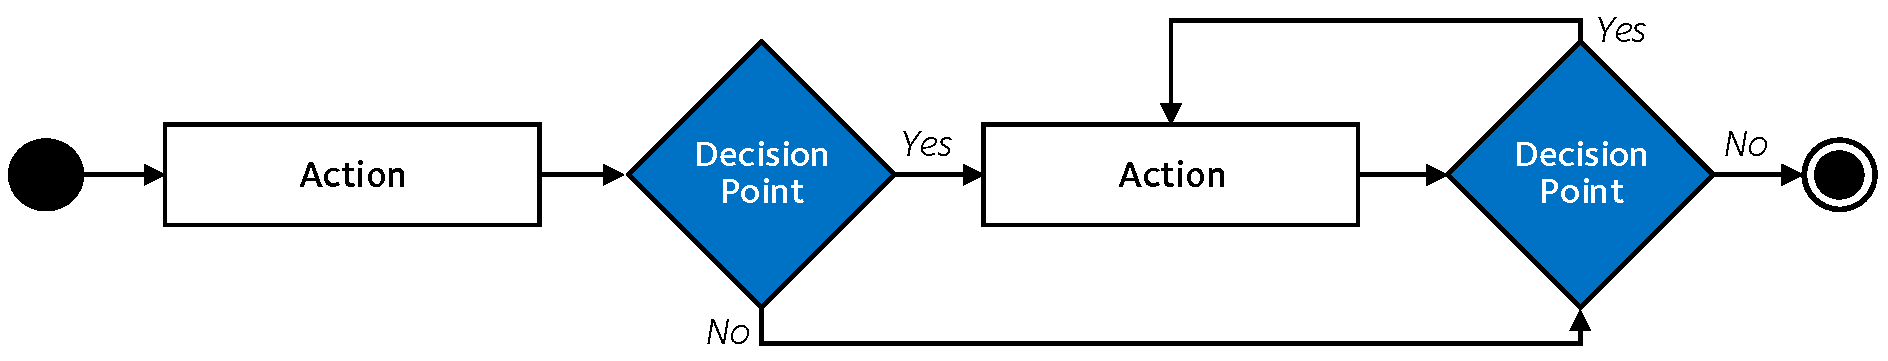
\includegraphics{figures/ch0-example.pdf}}
\end{figure*}

The sequence of events begins at the~
\includegraphics[height=\fontcharht\font`\d]{figures/ch0-example-start.pdf} and ends at the~
\includegraphics[height=\fontcharht\font`\d]{figures/ch0-example-end.pdf}.\footnote{Note that these symbols are not part of the \href{https://www.iso.org/standard/11955.html}{\texttt{ISO 5807:1985}} standard; they are part of the \emph{Unified Modelling Language (UML)} specification and have been included to ensure diagrams are simple to understand.} Diagram flow can be deduced by examining the direction of the arrows. Actions (or events) are denoted by the text contained within unfilled rectangles~
\includegraphics[height=\fontcharht\font`\d]{figures/ch0-example-action.pdf}, with decision points represented as~
\includegraphics[height=\fontcharht\font`\d]{figures/ch0-example-decision.pdf}. The different outcomes of decisions are denoted by the \emph{italicised} text at each output point of a~
\includegraphics[height=\fontcharht\font`\d]{figures/ch0-example-decision.pdf}.}
\end{itemize}

\glsreset{acr:url}

% While all figures are specially created for use in this thesis, several diagrams are based upon the figures provided in other publications. Where this is the case, acknowledgement of the source publication is included in the relevant figure caption. Permission was sought to include these figures wherever possible. Several vector artwork images have also been procured from \texttt{freepik.com} for non-commercial use.


\noindent\blueboxbold{Use of Illustrations}
Illustrations are used extensively to make the process of reading this thesis a little more enjoyable, as well as (hopefully) better demonstrating points and concepts being conveyed. While the author of this thesis drew a majority of the illustrations in \emph{Adobe \textregistered~Illustrator \textregistered~CS6}, free, pre-made vector artworks have also been downloaded from \texttt{freepik.com} and incorporated within illustrations. This statement serves as an acknowledgement that such artworks have been used and are included on the assumption that no part of this work will be used for commercial purposes.

\noindent\blueboxbold{Document Compilation, Rules and Regulations}
This thesis is typeset using \XeTeX, version \texttt{3.14159265-2.6-0.99999}. A custom \TeX\ class (\texttt{.cls}) has been developed and used for typesetting. The layout meets University of Glasgow PhD thesis regulations; core requirements of margins, font sizes and line spacing are fully complied with.

\end{preamble}

\newpage
\thispagestyle{empty}
\mbox{}
\newpage
\thispagestyle{empty}
\mbox{}
\newpage